



%前言:
% 时间序列分析需要判断序列的基本特性,包括随 机性的识别、平稳性的识别、趋势性的识别和周 期性的识别。
% p为了识别这些基本特性,人们发明了多种检测判 据。常用的判据有两种:
% p一是自相关系数;
% p二是Box-Pierce 的Q统计量和Box-Ljung修正的Q
% 统计量。
% p在时间序列的长度不是很大的情况下,采用Box- Ljung的修正Q统计量更为可靠
% 现实中的时间序列特性多是不同性质的叠加结果, 可能是趋势性、周期性和随机性的叠加,也可能是 趋势性、周期性和随机性的乘积或者迭代结果。
% p因此,地理学家的时间序列经常是一种复杂、丰富 多彩的研究对象。
% p在这种情况下,简单的时间序列判据无济于事,我 们需要更为复杂一些的研究方法,这就涉及后面讨 论的自相关分析和功率谱分析。






\section{时间序列的定义}

如果对地理系统进行长期观测,每隔一定的时间作一个记录,则记录结果可以构成时间序列。根据观测指标的数量可分为:

\begin{itemize}
    \item \textbf{一元时间序列}:只针对某一个指标进行观测所得到的记录
    \item \textbf{多元时间序列}:同时观测多个指标形成的记录
\end{itemize}

因此,时间序列(time series)实际上就是将某个指标在不同时刻的不同数值,按照时间先后的顺序排列而成的数列。例如:

\[x_1, x_2, \ldots, x_t, \ldots, x_p\]

就是一个时间序列的符号表示。

\subsectiom{地理时间序列的分类与构成}
\begin{figure}[htbp]
    \centering
    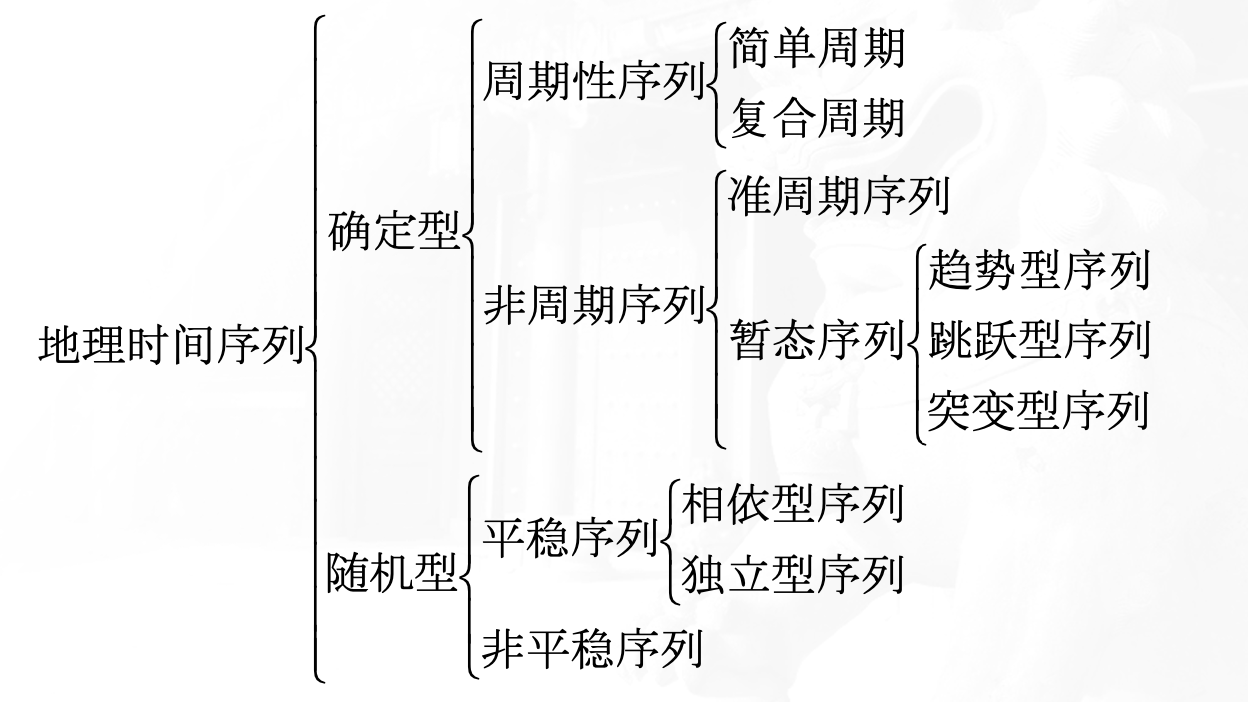
\includegraphics{figure/地理时间序列的分类与构成.png}
    \caption{时间序列示意图}
    \label{fig:timeseries}
\end{figure}


\section{时间序列的基本概念}

\subsection{时间序列的组成特征}
时间序列通常由以下几种变动特征共同作用构成:
\begin{itemize}
    \item 趋势变动(T): 表现为长期的增长或衰减趋势
    \item 循环变动(C): 包括周期性变动和季节性变动
    \item 不规则变动(I): 随机波动成分
\end{itemize}

\subsection{时间序列的数学表达}
时间序列可以用两种基本模型表示:
\begin{itemize}
    \item 加法模型: $Y = T + C + I$ (可分解)
    \item 乘法模型: $Y = T \times C \times I$ (难以分解)
\end{itemize}

\section{时间序列的周期性分析}

\subsection{周期类型}
\begin{itemize}
    \item 单一周期: 在地理研究中较为少见
    \item 多周期叠加: 
        \begin{itemize}
            \item 外在影响: 地球-太阳-月球相互作用
            \item 内在节律: 地理系统内部相互作用
        \end{itemize}
    \item 准周期(拟周期): 
        \begin{itemize}
            \item 形成原因: 多种周期成分不可通约性
            \item 典型案例: 太阳周期与地球周期引起的潮汐现象
        \end{itemize}
    \item 暂态序列: 无周期性,表现为趋势、跳跃或突变特征
\end{itemize}

\subsection{周期分析方法}
\begin{itemize}
    \item Fourier分析: 用于周期成分分解
    \item 不可通约性分析: 研究多周期叠加现象
\end{itemize}

\section{时间序列的变化特征}

\subsection{趋势性变化}
统计参数的系统性连续变化:
\begin{itemize}
    \item 均值变化
    \item 方差变化
    \item 协方差/相关系数变化
    \item 注: 变化源于系统自身性质,非随机抽样或观测误差
\end{itemize}

\subsection{突变性变化}
\begin{itemize}
    \item 跳跃(Phase Transition):
        \begin{itemize}
            \item 系统状态的急剧转变
            \item 统计参数发生不连续变化
        \end{itemize}
    \item 突变(Catastrophe):
        \begin{itemize}
            \item 跳跃的特殊形式
            \item 特点: 变化后系统趋于原状复归
        \end{itemize}
\end{itemize}

\section{随机过程基础}

\subsection{随机序列分类}
\begin{itemize}
    \item 平稳随机序列:
        \begin{itemize}
            \item 相依随机序列: 序列间存在相关性
            \item 独立随机序列: 纯随机,各时刻变量互不相关
        \end{itemize}
    \item 非平稳随机序列
\end{itemize}

\subsection{随机过程的数学描述}
\begin{itemize}
    \item 随机变量特征分析
    \item 自相关分析:
        \begin{itemize}
            \item 时间序列自相关: 如自回归模型(AR)、自回归-移动平均模型(ARMA)
            \item 空间自相关: 如Moran's I指数
        \end{itemize}
\end{itemize}




\section{自相关系数}

自相关系数是时间序列分析最基本的测度,其计算公式可以表示为:

\begin{equation}
\rho_\tau = \frac{\sum_{t=1}^{n-\tau}(x_t - \bar{x})(x_{t+\tau} - \bar{x})}{\sum_{t=1}^{n}(x_t - \bar{x})^2}
\end{equation}

式中:
\begin{itemize}
    \item $t$ 为时序
    \item $\tau$ 为时滞(time-lag,也可译为"时移"、"滞后"、"时间延迟"等)
    \item 一般取 $\tau = 1, 2, ..., n/4$
\end{itemize}


\begin{remark}
我的理解:
自相关系数实际上就是一个序列与其自身在不同时间点上的皮尔逊相关系数。它衡量了序列在不同时间点之间的线性相关程度。比如:
\begin{itemize}
    \item 当$\tau=1$时,计算的是相邻时刻的相关性
    \item 当$\tau=2$时,计算的是间隔1个时刻的相关性
    \item 以此类推
\end{itemize}
这种相关性分析有助于我们发现序列中的周期性模式和时间依赖关系。

其中皮尔逊相关系数的定义为:
\begin{equation}
r = \frac{\sum_{i=1}^n(x_i-\bar{x})(y_i-\bar{y})}{\sqrt{\sum_{i=1}^n(x_i-\bar{x})^2}\sqrt{\sum_{i=1}^n(y_i-\bar{y})^2}}
\end{equation}

皮尔逊相关系数衡量了两个变量之间的线性相关程度,取值范围为[-1,1]:
\begin{itemize}
    \item r=1表示完全正相关
    \item r=-1表示完全负相关
    \item r=0表示不相关
\end{itemize}
\end{remark}


\section{Q统计量及其修正}

为了利用自相关系数判断时间序列的基本特征,Box和Pierce提出了Q统计量:

\begin{equation}
Q = n\sum_{\tau=1}^m R_\tau^2
\end{equation}

其中:
\begin{itemize}
    \item $n$ 为样本容量
    \item $m$ 为所计算的自相关系数个数
    \item $R_\tau$ 为时滞$\tau$的自相关系数
\end{itemize}

Q统计量近似服从自由度为$m$的$\chi^2$分布:
\begin{itemize}
    \item Q值越小,表示$m$个自相关系数同时为0的可能性越大
    \item 需要在给定显著性水平$\alpha$下与临界值$\chi_\alpha^2(m)$比较
\end{itemize}

\subsection{Box-Ljung修正}

由于Box-Pierce的Q统计量未考虑时滞的影响,Ljung和Box对其进行了加权修正:

\begin{equation}
Q = n(n+2)\sum_{\tau=1}^m \frac{R_\tau^2}{n-\tau}
\end{equation}

Box-Ljung统计量同样近似服从$\chi^2$分布,但效果更好。其等价检验判据是自相关系数的P值(sig.值),因为P值基于渐近卡方分布。

Q统计量的主要用途:
\begin{itemize}
    \item 检验时间序列是否为白噪声序列
    \item 判断时间序列模型的适当性
    \item 确定时间序列的相关性结构
\end{itemize}



\subsection{四种时间序列特性的对比}
\begin{figure}[htbp]
    \centering
    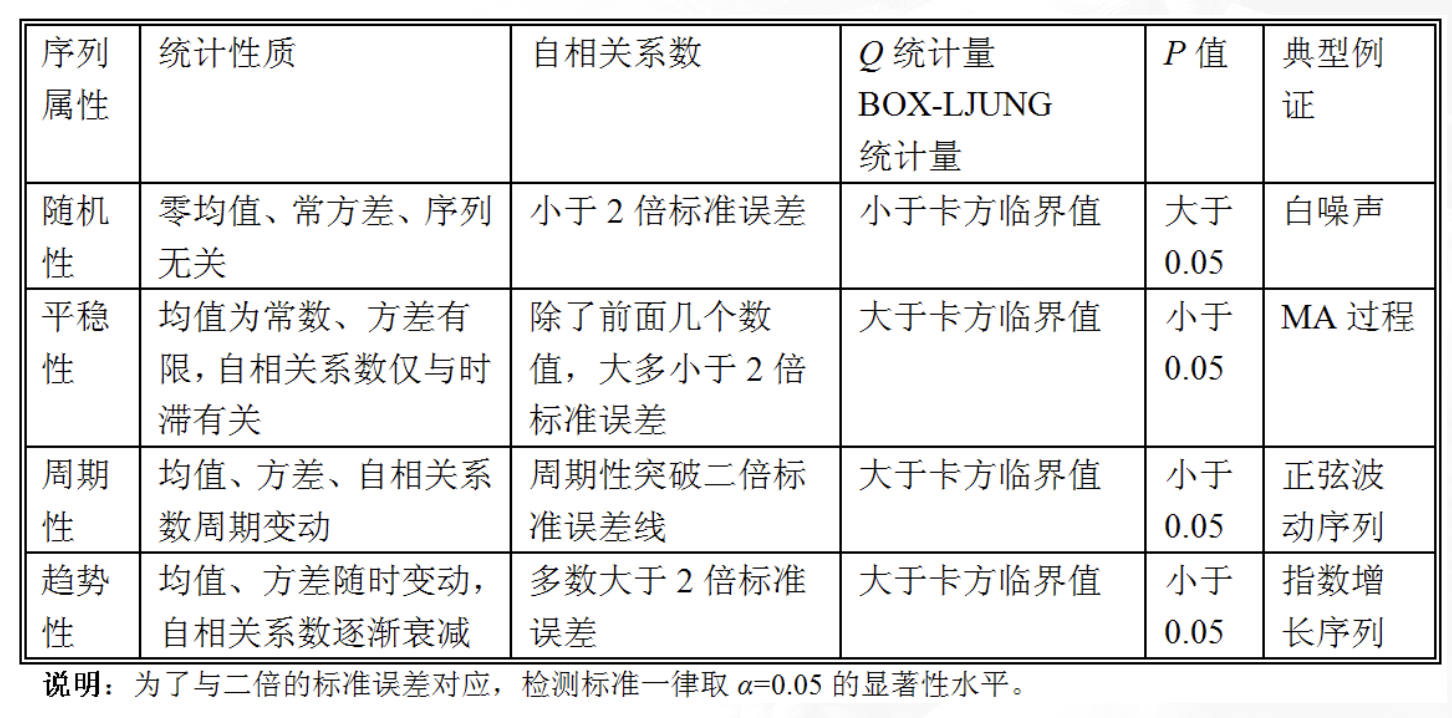
\includegraphics{figure/四种时间序列特性的对比.png}
    \caption{时间序列示意图}
    \label{fig:timeseries}
\end{figure}

可以看到,Q统计量检测效果与P值的检测效果一致:在一定的显著性水平下,Box-Ljung统计量是否小于卡方临界值与P值是否大于某个显著性水平是一个问题的两个方面。

第二个检测标准在理论上与P值是否大于或者小于某个显著性水平等价。但在现实中,由于序列结果的复杂性,我们需要结合Q统计量和P值共同判断。

% 具体来说:
% \begin{itemize}
%     \item 随机性序列: Q统计量较小,P值较大(>0.05)
%     \item 平稳性序列: Q统计量较大,P值较小(<0.05) 
%     \item 周期性序列: Q统计量较大,P值较小(<0.05),且自相关系数呈周期性变化
%     \item 趋势性序列: Q统计量很大,P值很小(<0.01),且自相关系数呈单调递减
% \end{itemize}

% 这四种特性并不是互斥的,实际的时间序列往往表现出多种特性的叠加。因此在分析时需要综合考虑各种统计指标,合理判断序列的主要特征。



\section{时间序列特征的识别}

时间序列特征的识别内容主要包括四个方面:随机性的识别、平稳性的识别、周期性的识别和趋势性的识别。下面将分别介绍这四种特征的识别方法。

\subsection{随机性的识别}
随机性是指将反映时间序列的样本路径$x_0、x_1、...、x_{t-1}、x_t$视为一组信号时,当前信号$x_t$与在此之前的所有信号之间完全独立。换言之,在已知$x_0、x_1、...、x_{t-1}$的条件下,$x_t$依然不可预测。随机性的要点包括三个方面:均值为零,方差为常数,序列不存在自相关(自协方差为零)。

随机性检验的一个定量判据是自相关系数,其方法与回归分析中的相关系数检验相似。一般认为,当取显著性水平为$\alpha=0.05$时,如果自相关系数满足:

\[-1.96 \leq R_\tau \leq 1.96/\sqrt{n}\]

则有95\%的把握断定所有的自相关系数与0没有显著性差异,从而该时间序列具有随机性。这里的1.96来自正态分布,是一个统计学常数,一般近似为2。

概括起来,当一个时间序列满足如下条件时,可认为它在某个显著性水平上是随机的:
\begin{enumerate}
    \item 自相关系数绝对值小于$1.96/\sqrt{n}$
    \item 统计量Q满足$Q < \chi^2$(显著性水平取0.05)
    \item P值(sig.值)大于0.05,典型的情况大于0.5
\end{enumerate}

\subsection{平稳性的识别}
时间序列的平稳性是指产生该时间序列的随机过程大体上以恒定的平均水平在整个时间序列内均衡发展,即数据整体是平稳的、没有明显跳跃或突变、整体都在大致水平上,且在平均水平上起伏的概率在各个时间点上都相同。换言之,一个严格的时间平稳序列的均值为常数,方差为有限值,不同观测之间的协方差仅依赖于观测值之间的时间滞后阶数。

当一个时间序列满足如下条件时,可认为它在某个显著性水平上是平稳的:
\begin{enumerate}
    \item 只有前面有限阶数的自相关系数绝对值大于二倍标准误差,后面的绝大多数自相关系数小于$1.96/\sqrt{n}$
    \item 统计量Q满足$Q \geq \chi^2$(显著性水平取0.05)
    \item P值(sig.值)小于0.05,典型的情况小于0.01
\end{enumerate}

值得注意的是,移动平均过程(MA过程)都是典型的平稳过程。

\subsection{周期性的识别}
周期变动序列常被视为广义的平稳序列的一类,因为从远距离看来,周期序列的变化曲线粗视化为一条水平线。周期序列的统计特性是:均值和方差为常数,自相关系数周期变动。

时间序列的周期性分为单向周期和双向周期两种情况:
\begin{itemize}
    \item 单向周期:指的是只有峰值或谷值的情况。如果一个时间序列周期性地出现某种脉动或者脉冲,就属于单向周期序列
    \item 双向周期:即周期波动,既有峰值又有谷值,如某海域海平面年均高度的自相关系数随时滞的变化曲线
\end{itemize}

周期序列的自相关系数序列具有如下特征:
\begin{enumerate}
    \item 自相关系数周期性地突破二倍标准误差(standard error)线
    \item Q统计量大于相应的卡方统计量的临界值(显著性水平取0.05)
    \item P值(sig.值)小于0.05,典型的情况小于0.01
\end{enumerate}

\subsection{趋势性的识别}
趋势序列的统计特性非常明显:均值和方差都随着计算的时间起点不同而改变,自相关系数单边衰减或者阻尼振动式衰减。具有趋势性的时间序列基本特征概括如下:
\begin{enumerate}
    \item 排列靠前的多个自相关系数突破二倍标准误差线,典型的趋势序列的自相关系数在有效时滞范围内都超过二倍的标准误差线
    \item Q统计量大于相应的卡方统计量的临界值(显著性水平取0.05)
    \item P值(sig.值)小于0.05,典型的情况小于0.01
\end{enumerate}



\textbf{重要:随机性是最为基本的特性。现实中的观测数据或多或少具有随机性。一个复杂的序列通常是包括随机性在内的多种属性的序列"组合"而成的结果。}

\textbf{特例:}
\textbf{需要特别说明的是周期性的统计性质。}

\textbf{一个典型的周期序列,其平均值围绕0或者某个平均值周期波动,但振幅较小,远距离看来可以视为常数;其方差围绕某个常数周期波动,可以看做有限;自相关系数随着时滞的改变而周期变动,这种周期性与计算的时间起点没有明确的关系。}

\textbf{因此,在不太严格的情况下,周期序列也可以视为平稳序列。但是,反过来,平稳序列却未必包含周期——严格意义的平稳序列可以视为周期无穷大,但这仅仅是理论上的一种处理技巧。}




P值基于渐近卡方近似,与Q统计量的检验相辅相 成:如果一个序列是随机的,则其自相关系数的P 值大于0.05,典型情况大于0.5。
p反之,如果一个序列不是随机的,则其自相关系 数序列的P值小于0.05,典型情况小于0.01。


\section{第一节:协方差平稳的时间序列}

\begin{table}[htbp]
    \centering
    \begin{tabular}{|p{2.5cm}|p{5cm}|p{5cm}|}
    \hline
    \rowcolor{lightblue}
    \textbf{场景} & \textbf{理论(推理)} & \textbf{经验(应用)} \\
    \hline
    \rowcolor{lightgray}
    统计分析 & 
    总体(population) \newline
    例:某城市所有居民的年收入分布服从正态分布 $N(\mu, \sigma^2)$ & 
    样本(sample) \newline
    例:随机抽取1000名居民的收入数据进行分析 \\
    \hline
    \rowcolor{lightgreen}
    现实情况 & 
    随机过程(stochastic process) \newline
    例:协方差平稳的时间序列 $\{X_t\}$,从无限远过去延伸到无限远将来 & 
    实现(realization) \newline
    例:某个随机过程的一次完整实现 $\{..., x_{-2}, x_{-1}, x_0, x_1, x_2, ...\}$ \\
    \hline
    \rowcolor{lightgreen}
    时间序列分析 & 
    实现(realization) \newline
    例:理论上完整的时间序列实现 $\{x_t\}_{t=-\infty}^{\infty}$ & 
    样本路径(sample path) \newline
    例:实际观测到的有限长度序列 $\{x_1, x_2, ..., x_T\}$ \\
    \hline
    \end{tabular}
    \caption{统计学概念对应关系及例子}
    \label{tab:stats-concepts-examples}
\end{table}


让我们用一个简单的天气温度预测的例子来说明:

\subsection*{随机过程 (Stochastic Process)}
考虑北京24小时的气温变化预测:
\begin{itemize}
    \item 数学表达:$\{X(t), t \in [0, 24]\}$,其中$X(t)$是$t$时刻的温度
    \item 每个时刻的温度都是随机变量
    \item 包含所有可能的温度变化路径
    \item 可用数学模型描述:
    \begin{itemize}
        \item 均值函数:$\mu(t) = 20 + 5\sin(\pi t/12)$ °C
        \item 加上随机波动:$dX(t) = \mu(t)dt + \sigma dW(t)$
    \end{itemize}
\end{itemize}

\subsection*{实现 (Realization)}
是随机过程的一次具体表现:
\begin{itemize}
    \item 例如2024年1月28日的实际温度记录:
    \begin{itemize}
        \item 凌晨0点:5°C
        \item 早上6点:3°C
        \item 中午12点:8°C
        \item 晚上6点:6°C
        \item 晚上11点:4°C
    \end{itemize}
    \item 这只是众多可能路径中的一条
\end{itemize}

简而言之:
\begin{itemize}
    \item 随机过程:所有可能温度变化的数学描述
    \item 实现:实际观测到的一条温度变化曲线
\end{itemize}



\section{第二节: 协方差平稳性质}


\subsection{研究原因}
分析时间序列的协方差平稳性质是非常重要的。这是因为时间序列分析的主要目标是对未来进行预测,而协方差平稳性保证了序列在不同时间段具有相似的统计特性。只有当序列具有协方差平稳性时,基于历史数据建立的预测模型才能有效应用于未来。如果序列不具备协方差平稳性,意味着未来的统计特性与过去不同,预测将失去可靠性。


\subsection{自协方差的定义}
对于时间序列$\{X_t\}$,其自协方差函数定义为:
\begin{equation}
\gamma(t, \tau) = Cov(X_t, X_{t+\tau}) = E[(X_t - \mu)(X_{t+\tau} - \mu)]
\end{equation}

其中:
\begin{itemize}
    \item $Cov$表示协方差
    \item $E$表示期望值
    \item $\mu$是均值
    \item $\tau$是时滞
\end{itemize}


让我们以每日气温序列为例来理解自协方差的物理意义:

\subsection{气温序列自协方差计算示例}
假设我们有一个城市10天的日均气温序列(单位:℃):
\begin{itemize}
    \item 序列值: [20, 22, 21, 23, 22, 21, 20, 22, 21, 20]
    \item 均值$\mu = 21.2$℃
\end{itemize}

让我们计算$\tau = 1$时的自协方差$\gamma(1)$:

1. 首先计算每个时刻与均值的偏差$(X_t - \mu)$:
\begin{align*}
    X_1 - \mu &= 20 - 21.2 = -1.2 \\
    X_2 - \mu &= 22 - 21.2 = 0.8 \\
    X_3 - \mu &= 21 - 21.2 = -0.2 \\
    X_4 - \mu &= 23 - 21.2 = 1.8 \\
    X_5 - \mu &= 22 - 21.2 = 0.8 \\
    X_6 - \mu &= 21 - 21.2 = -0.2 \\
    X_7 - \mu &= 20 - 21.2 = -1.2 \\
    X_8 - \mu &= 22 - 21.2 = 0.8 \\
    X_9 - \mu &= 21 - 21.2 = -0.2 \\
    X_{10} - \mu &= 20 - 21.2 = -1.2
\end{align*}

2. 计算相邻时刻偏差的乘积$(X_t - \mu)(X_{t+1} - \mu)$:
\begin{align*}
    t=1: &(-1.2)(0.8) = -0.96 \\
    t=2: &(0.8)(-0.2) = -0.16 \\
    t=3: &(-0.2)(1.8) = -0.36 \\
    t=4: &(1.8)(0.8) = 1.44 \\
    t=5: &(0.8)(-0.2) = -0.16 \\
    t=6: &(-0.2)(-1.2) = 0.24 \\
    t=7: &(-1.2)(0.8) = -0.96 \\
    t=8: &(0.8)(-0.2) = -0.16 \\
    t=9: &(-0.2)(-1.2) = 0.24
\end{align*}

3. 取这些乘积的平均值得到$\gamma(1)$:
$$\gamma(1) = \frac{1}{9}\sum_{t=1}^9(X_t - \mu)(X_{t+1} - \mu) = \frac{-0.96-0.16-0.36+1.44-0.16+0.24-0.96-0.16+0.24}{9} = -0.0933$$

这个负的自协方差值表明:
\begin{itemize}
    \item 当某一天气温高于平均值21.2℃时,第二天气温倾向于低于平均值
    \item 当某一天气温低于平均值21.2℃时,第二天气温倾向于高于平均值
    \item 自协方差值-0.0933表示相邻两天气温具有弱的负相关性
\end{itemize}
这种弱负相关性可能反映了温度的小幅波动特性:如果今天气温偏高,明天可能会稍微回落;如果今天气温偏低,明天可能会稍微回升。但由于相关性很弱(接近0),这种模式并不明显。



\section{协方差平稳的三个数学特征}

\subsection{为什么需要这三个特征?}
在研究时间序列时,我们的主要目标是利用历史数据预测未来。要实现这一目标,序列必须具有某种"稳定性"。这种稳定性体现在三个方面:
\begin{itemize}
    \item 序列的整体水平应该保持稳定(均值平稳)
    \item 序列的波动模式应该保持稳定(协方差平稳)
    \item 序列的波动幅度应该有界(有限方差)
\end{itemize}

让我们通过一个具体的例子来理解这三个特征:某城市2023年1月的日均气温数据。

\subsection{特征一:均值平稳性}
\subsubsection{直观理解}
均值平稳性要求序列在任何时间点的期望值都相同。就像一个城市的1月份气温,虽然每天都在波动,但整体水平应该保持在一个相对稳定的范围内。

\subsubsection{数学表达}
对于时间序列 $\{X_t\}$,要求:
$$E(X_t) = \mu, \quad \forall t$$

\subsubsection{实例分析}
考虑以下两种温度序列:
\begin{itemize}
    \item 平稳序列:$T_t = 5 + \epsilon_t$,其中$\epsilon_t \sim N(0,1)$
    每天气温在5℃附近随机波动,均值恒为5℃
    
    \item 非平稳序列:$T_t = 5 + 0.2t + \epsilon_t$
    由于加入了时间趋势$0.2t$,温度会持续上升,均值不再恒定
\end{itemize}

\subsection{特征二:协方差平稳性}
\subsubsection{直观理解}
协方差平稳性要求序列的相关结构保持稳定。以气温为例,如果今天和明天的气温关系在月初和月末应该保持类似的模式。

\subsubsection{数学表达}
对于任意时间点$t$和时间间隔$\tau$:
$$\gamma(t,\tau) = Cov(X_t, X_{t+\tau}) = E[(X_t-\mu)(X_{t+\tau}-\mu)] = \gamma(\tau)$$

重要性质:
\begin{itemize}
    \item 对称性:$\gamma(\tau) = \gamma(-\tau)$
    意味着向前看τ天和向后看τ天的关系相同
    
    \item 特殊情况:$\gamma(0) = Var(X_t)$
    当时间间隔为0时,自协方差即为方差
\end{itemize}

\subsubsection{实例分析}
对于气温序列,计算1天间隔的自协方差:
$$\gamma(1) = E[(T_t-\mu)(T_{t+1}-\mu)]$$

例如,连续三天的温度:
\begin{itemize}
    \item 第一天:4℃ (低于均值)
    \item 第二天:4.5℃ (仍低于均值)
    \item 第三天:5.5℃ (高于均值)
\end{itemize}

这种模式在月内任何时候都应该保持类似的统计特征。

\subsection{特征三:有限方差}
\subsubsection{直观理解}
有限方差要求序列的波动幅度不会无限增大。就像气温波动,虽然每天都在变化,但不会出现无限大的波动。

\subsubsection{数学表达}
要求:
$$\gamma(0) = Var(X_t) < \infty$$
且
$$|\gamma(\tau)| \leq \gamma(0)$$

\subsubsection{实例分析}
以下两种气温模型:
\begin{itemize}
    \item 合理模型(有限方差):
    $$T_t = 5 + \epsilon_t, \quad \epsilon_t \sim N(0,1)$$
    温度的波动范围基本在$[2,8]$之间,方差有限。
    
    \item 不合理模型(方差无限):
    $$T_t = T_{t-1} + \epsilon_t$$
    这种模型允许温度无限累积,不符合实际。
\end{itemize}

\section{完整实例分析}
让我们看一个完整的10天气温序列:
$$[4.8, 5.2, 4.9, 5.3, 5.1, 4.7, 5.0, 5.4, 4.8, 5.2]$$

1. 均值平稳性检验:
   - 计算均值:$\mu = 5.04$
   - 数据始终在5℃附近波动,无明显趋势

2. 协方差平稳性检验:
   - 计算1天间隔自协方差
   - 验证在不同时间段的自协方差是否稳定

3. 有限方差检验:
   - 计算样本方差:约为0.05
   - 确认波动范围有界:$[4.7, 5.4]$

这个序列满足所有三个特征,因此是协方差平稳的。



\textbf{为什么要保证$|\gamma(\tau)| \leq \gamma(0)$?}

$\gamma(0)$ 是序列与自身的协方差,也就是序列的方差
$\gamma(\tau)$ 是序列与其滞后τ期的协方差
这个不等式告诉我们:\textbf{任何时间间隔的自协方差的绝对值都不能超过序列自身的方差}

\begin{itemize}
    \item 从统计学角度:如果某个时间间隔的自协方差大于方差,这意味着序列与其滞后值的关系比与自身的关系还要强,这在统计上是不合理的
    \item 从物理意义:一个变量与自身的关联度应该是最强的,与其他时刻的关联度应该随着时间间隔的增加而减弱
    \item 从预测角度:如果不满足这个条件,预测模型可能会产生不稳定的结果,导致预测误差无限放大
\end{itemize}



\subsection{协方差平稳序列的处理}

可以看到,协方差平稳序列的条件十分苛刻,现实中的样本路径一般很难满足上述全部条件。时间序列的观测值通常以各种方式破坏了时间序列的协方差平稳性。

在这种情况下,有必要对时间序列进行适当地处理。处理方法大致可以分为两类:
\begin{itemize}
    \item 序列分解
    \item 序列变换
\end{itemize}

\subsubsection{序列分解}
现实中的时间序列之所以复杂,是因为它们通常是多种序列成分的复合(叠加或者乘积)。我们可以通过时间序列的分解进行平稳化处理,剔除其中容易开展预测分析的趋势性、季节性成分,保留其中满足协方差平稳性的周期成分或者随机成分,然后建立模型。

\subsubsection{序列变换}
最常见的序列变换是差分。有很多时间序列本身协方差并不平稳,但其增长率却是协方差平稳的,在这种情况下可以基于差分建模。例如,双重差分DID模型就是利用这个原理。



\section{协方差平稳序列的处理方法示例}

\subsection{1. 序列分解示例:零售销售数据}
考虑某商店2023年的月度销售额(万元)数据:
$$[82, 85, 90, 120, 150, 160, 180, 190, 150, 100, 90, 150]$$

这个序列明显不满足协方差平稳性,因为它包含了多个成分:

1. \textbf{趋势成分}:
   - 基础销售额逐月增长趋势
   - 可以用线性回归估计:$T_t = 80 + 5t$

2. \textbf{季节性成分}:
   - 暑期(7-8月)销售额明显高于其他月份
   - 春节(1月)销售额较低
   - 季节指数:$S_t = [0.9, 0.9, 1.0, 1.2, 1.3, 1.4, 1.5, 1.5, 1.2, 1.0, 0.9, 1.2]$

3. \textbf{随机成分}:
   - 剔除趋势和季节性后的残差
   - $R_t = X_t - T_t - S_t$

分解后,我们可以重点分析随机成分$R_t$,它通常更接近协方差平稳序列。

\subsection{2. 序列变换示例:股票价格数据}
考虑某股票连续5个交易日的收盘价(元):
$$[50, 52, 55, 53, 56]$$

这个价格序列本身不是协方差平稳的,因为:
\begin{itemize}
    \item 均值不稳定:价格整体呈上升趋势
    \item 方差可能随时间变化:波动幅度可能增大
\end{itemize}

\textbf{一阶差分变换}:
计算相邻两天的价格变化:
\begin{align*}
    \Delta P_1 &= 52 - 50 = 2 \\
    \Delta P_2 &= 55 - 52 = 3 \\
    \Delta P_3 &= 53 - 55 = -2 \\
    \Delta P_4 &= 56 - 53 = 3
\end{align*}

差分后的序列$[2, 3, -2, 3]$更接近协方差平稳:
\begin{itemize}
    \item 均值接近于常数(日均变化约1.5元)
    \item 波动幅度相对稳定(在±3元范围内)
\end{itemize}

\subsection{3. 复杂示例:GDP增长数据}
考虑某国季度GDP数据(亿元):
$$[1000, 1100, 1250, 1300, 1150, 1280, 1450, 1500]$$

这个序列同时存在多个非平稳特征:
\begin{itemize}
    \item 长期增长趋势
    \item 季节性波动(第四季度通常最高)
    \item 波动幅度随基数增大而增大
\end{itemize}

\textbf{处理步骤}:

1. \textbf{对数变换}:
   先取对数处理异方差性:
   $$[\ln(1000), \ln(1100), ..., \ln(1500)]$$

2. \textbf{季节性调整}:
   计算每个季度的季节指数,并除去季节性影响

3. \textbf{差分处理}:
   对调整后的序列进行差分,得到增长率序列

最终得到的序列更接近协方差平稳,可以用于建模预测。

\section{处理方法的选择原则}

1. \textbf{序列分解适用于}:
\begin{itemize}
    \item 具有明显周期性或季节性的数据
    \item 可以清晰识别不同成分的序列
    \item 例如:零售销售、旅游人数、农产品价格
\end{itemize}

2. \textbf{序列变换适用于}:
\begin{itemize}
    \item 具有持续增长趋势的数据
    \item 波动幅度随时间变化的序列
    \item 例如:股票价格、GDP、人口数据
\end{itemize}

3. \textbf{混合方法适用于}:
\begin{itemize}
    \item 同时具有多种非平稳特征的复杂序列
    \item 需要多步处理才能达到平稳的数据
    \item 例如:宏观经济指标、跨年度财务数据
\end{itemize}




\section{自相关函数与偏自相关函数}

\subsection{1. 自相关函数(ACF)}

\subsubsection{基本概念}
自相关函数描述了时间序列中不同时刻观测值之间的线性相关关系。其核心思想是:
\begin{itemize}
    \item 测量序列中任意两个时点的观测值之间的相关程度
    \item 反映过去的随机冲击(shock)对未来的影响程度
\end{itemize}

\subsubsection{数学定义}
自相关系数的计算公式:
$$\rho(\tau) = \frac{\gamma(\tau)}{\gamma(0)} = \frac{Cov(x_t, x_{t-\tau})}{Var(x_t)}$$

其中:
\begin{itemize}
    \item $\tau$ 是时间间隔(时滞)
    \item $\gamma(\tau)$ 是自协方差函数
    \item $\gamma(0)$ 是序列的方差
\end{itemize}

\subsubsection{特点}
1. $\rho(0) = 1$ (序列与自身的相关系数为1)
2. $|\rho(\tau)| \leq 1$ (自相关系数的绝对值不超过1)
3. $\rho(\tau) = \rho(-\tau)$ (对称性)

\subsection{2. 偏自相关函数(PACF)}

\subsubsection{基本概念}
偏自相关函数衡量了在去除中间时期影响后,两个时点观测值之间的"纯"相关关系。

\subsubsection{数学表达}
对于时滞$\tau$,偏自相关是下面回归方程中的$p_{\tau}$:
$$x_t = p_0 + p_1x_{t-1} + p_2x_{t-2} + ... + p_{\tau}x_{t-\tau} + \epsilon_t$$

\subsection{3. 实例分析:月度销售数据}
考虑某商店12个月的销售数据(万元):
$$[100, 120, 115, 125, 110, 105, 130, 140, 120, 110, 105, 125]$$

\subsubsection{ACF分析}
计算不同时滞的自相关系数:
\begin{align*}
\rho(1) &= 0.65 \text{ (相邻月份的关联度)} \\
\rho(2) &= 0.45 \text{ (间隔一个月的关联度)} \\
\rho(3) &= 0.20 \text{ (间隔两个月的关联度)}
\end{align*}

解读:
\begin{itemize}
    \item 相邻月份销售额的相关性最强
    \item 随着时间间隔增加,相关性逐渐减弱
    \item 体现了"近期影响大,远期影响小"的特点
\end{itemize}

\subsubsection{PACF分析}
计算偏自相关系数:
\begin{align*}
p(1) &= 0.65 \text{ (直接影响)} \\
p(2) &= 0.20 \text{ (去除1阶影响后的相关性)} \\
p(3) &= 0.05 \text{ (去除1、2阶影响后的相关性)}
\end{align*}

解读:
\begin{itemize}
    \item $p(1)$显著,说明上个月的销售直接影响本月
    \item $p(2)$较小,说明两个月前的影响主要是通过上个月间接传导
    \item $p(3)$接近0,说明三个月前基本没有直接影响
\end{itemize}

\subsection{4. ACF与PACF的区别}

1. \textbf{测量角度}:
\begin{itemize}
    \item ACF:测量总体相关性,包括直接和间接影响
    \item PACF:仅测量直接相关性,剔除了中间时期的影响
\end{itemize}

2. \textbf{应用价值}:
\begin{itemize}
    \item ACF:帮助识别时间序列的整体依赖结构
    \item PACF:帮助确定自回归模型的阶数
\end{itemize}

3. \textbf{实际应用}:
\begin{itemize}
    \item 两个函数通常结合使用
    \item 相互补充,共同提供序列特征的完整信息
\end{itemize}

\subsection{5. 在ARIMA模型中的应用}

1. \textbf{模型识别}:
\begin{itemize}
    \item ACF快速衰减,PACF截尾:暗示AR模型
    \item ACF截尾,PACF快速衰减:暗示MA模型
    \item 两者都缓慢衰减:暗示ARMA模型
\end{itemize}

2. \textbf{阶数确定}:
\begin{itemize}
    \item AR模型:通过PACF的截尾位置确定阶数
    \item MA模型:通过ACF的截尾位置确定阶数
\end{itemize}



% 这个介绍:
\section{MA(1)过程介绍}
移动平均模型的基本思想是假定时间序列的所有变动都是由各种冲击造成的,这些冲击表现为误差项(error term)。

\subsection{实际应用示例}
以一个区域的气候为例:
\begin{itemize}
    \item 连续多年的年降雨量可以构成一个时间序列的样本数据
    \item 根据传统观点,区域气候的变化是平稳的
    \item 某些年份的干旱和洪涝是随机冲击形成的扰动(气候异常)
    \item 一定时间后气候变化会恢复稳定(回归正常)
\end{itemize}

\section{MA(q)过程}
\subsection{基本定义}
MA(1)过程可以推广到一般形式,即MA(q)过程。q阶移动平均模型可以表示为:

\[x_t = e_t + \theta_1e_{t-1} + \theta_2e_{t-2} + ... + \theta_qe_{t-q}\]
其中:\[e_t \sim WN(0,\sigma^2)\]

\subsection{MA(2)示例}
以q=2为例,MA(2)过程可以表示为:
\[x_t = e_t + \theta_1e_{t-1} + \theta_2e_{t-2}\]

变形后可得:
\[e_t = x_t - \theta_1e_{t-1} - \theta_2e_{t-2}\]

\subsection{MA(q)过程的特性}
\begin{itemize}
\item 具有更丰富的动态模式,可以提高分析精确性
\item 有限阶MA(q)过程是协方差平稳的
\item 具有长程记忆(long memory)特性,通过自相关函数反映
\item 在时滞大于q时,自相关函数与0没有显著差异(q阶截尾)
\item 偏相关函数通常呈现逐渐衰减特征,可能出现阻尼振荡
\end{itemize}


\section{应用价值}
相对于MA(1)过程:
\begin{itemize}
    \item MA(q)过程可以更好地近似Wold表示
    \item 主要困难在于需要估计更多的参数
\end{itemize}


\section{自回归过程 AR}
\subsection{AR(1)过程介绍}
自回归过程是Wold表示的另一种自然近似。其基本特点:
\begin{itemize}
    \item 可以视为一种随机差分方程
    \item 是对离散时间序列动态建模的有效工具
    \item 基本策略是将序列的现期值表示为序列过去的观察值加上随机冲击
\end{itemize}

\subsection{AR(p)过程定义}
将1阶自回归推广到一般形式,得到p阶自回归AR(p)过程:

\[x_t = \phi_1x_{t-1} + \phi_2x_{t-2} + ... + \phi_px_{t-p} + e_t\]
其中:\[e_t \sim WN(0,\sigma^2)\]

\subsection{AR(p)过程的统计性质}
AR(p)过程具有以下主要特性:
\begin{itemize}
    \item \textbf{平稳性条件}:
        \begin{itemize}
            \item 特征方程的根必须在单位圆之外
            \item AR(1)情况下要求|\phi_1| < 1
        \end{itemize}
    \item \textbf{自相关函数特征(ACF)}:
        \begin{itemize}
            \item 呈现指数衰减或震荡衰减
            \item 理论上延伸至无穷,但实际中通常在较大时滞后可忽略
        \end{itemize}
    \item \textbf{偏自相关函数(PACF)}:
        \begin{itemize}
            \item 在滞后p之后截尾(p阶截尾)
            \item 这是识别AR过程阶数的重要特征
        \end{itemize}
\end{itemize}

\subsection{与MA过程的比较}
AR(p)和MA(q)过程的主要区别:
\begin{itemize}
    \item AR过程依赖于过去的观测值,MA过程依赖于过去的随机冲击
    \item AR过程的自相关函数拖尾,MA过程的自相关函数截尾
    \item AR过程的偏自相关函数截尾,MA过程的偏自相关函数拖尾
    \item AR过程需要满足平稳性条件,MA过程总是平稳的
\end{itemize}


% 这里补充单位根的证明; 


\section{自回归移动平均模型 ARMA}
\subsection{ARMA(p,q)过程的定义}
ARMA过程将自回归过程和移动平均过程集成在同一个模型中。ARMA(p,q)过程的一般形式为:

\[x_t = \phi_1x_{t-1} + \phi_2x_{t-2} + ... + \phi_px_{t-p} + e_t + \theta_1e_{t-1} + \theta_2e_{t-2} + ... + \theta_qe_{t-q}\]

其中:
\begin{itemize}
    \item p是自回归项的阶数
    \item q是移动平均项的阶数
    \item \(\phi_i\)是自回归系数
    \item \(\theta_j\)是移动平均系数
    \item \(e_t \sim WN(0,\sigma^2)\)
\end{itemize}

\subsection{滞后算子表示}
使用滞后算子L,ARMA(p,q)过程可以简洁地表示为:

\[\phi(L)x_t = \theta(L)e_t\]

其中:
\[\phi(L) = 1 - \phi_1L - \phi_2L^2 - ... - \phi_pL^p\]
\[\theta(L) = 1 + \theta_1L + \theta_2L^2 + ... + \theta_qL^q\]

\subsection{平稳性与可逆性}
\subsubsection{平稳性条件}
ARMA过程的平稳性主要由其AR部分决定:
\begin{itemize}
    \item 特征方程\[\phi(z) = 1 - \phi_1z - \phi_2z^2 - ... - \phi_pz^p = 0\]的所有根必须位于单位圆之外
    \item 这确保了过程的长期稳定性
\end{itemize}

\subsubsection{可逆性条件}
可逆性主要由MA部分决定:
\begin{itemize}
    \item 特征方程\[\theta(z) = 1 + \theta_1z + \theta_2z^2 + ... + \theta_qz^q = 0\]的所有根必须位于单位圆之外
    \item 可逆性确保了当前观测值对过去冲击的依赖程度随时间衰减
\end{itemize}

\subsection{ARMA过程的统计性质}
\subsubsection{均值与方差}
当ARMA过程平稳时:
\begin{itemize}
    \item 期望:E(x_t) = 0
    \item 方差:\[\gamma(0) = \sum_{j=0}^{\infty}\psi_j^2\sigma_e^2\]
    其中\(\psi_j\)是MA(∞)表示中的系数
\end{itemize}

\subsubsection{自相关函数}
ARMA(p,q)过程的自相关函数:
\begin{itemize}
    \item 对k > q,满足p阶差分方程:
    \[\rho_k = \phi_1\rho_{k-1} + \phi_2\rho_{k-2} + ... + \phi_p\rho_{k-p}\]
    \item 呈现混合性质:初始q+1个自相关系数反映MA和AR的共同影响,之后仅反映AR特征
\end{itemize}

\subsubsection{偏自相关函数}
ARMA过程的偏自相关函数:
\begin{itemize}
    \item 不像纯AR或纯MA过程那样具有明确的截尾性质
    \item 表现为渐近衰减特征
    \item 衰减模式可能是指数型或振荡型
\end{itemize}

\subsection{模型识别}
ARMA模型的阶数识别主要基于:
\begin{itemize}
    \item 自相关函数(ACF)分析
    \item 偏自相关函数(PACF)分析
    \item 信息准则(如AIC、BIC等)
    \item 残差白噪声检验
\end{itemize}

\subsection{估计与预测}
\subsubsection{参数估计方法}
主要的估计方法包括:
\begin{itemize}
    \item 最小二乘估计(LSE)
    \item 最大似然估计(MLE)
    \item 矩估计法
    \item 条件最小二乘估计
\end{itemize}

\subsubsection{预测}
\begin{itemize}
    \item 最小均方误差预测
    \item h步向前预测公式:
    \[\hat{x}_{t+h} = \phi_1\hat{x}_{t+h-1} + ... + \phi_p\hat{x}_{t+h-p} + \theta_1e_{t+h-1} + ... + \theta_qe_{t+h-q}\]
    \item 预测误差随预测期限的增加而增大
\end{itemize}

\section{模型的实际应用}
\subsection{模型选择步骤}
1. 数据预处理
   \begin{itemize}
       \item 平稳性检验
       \item 季节性调整
       \item 趋势去除
   \end{itemize}

2. 模型识别
   \begin{itemize}
       \item ACF/PACF图分析
       \item 信息准则比较
   \end{itemize}

3. 参数估计
   \begin{itemize}
       \item 选择适当的估计方法
       \item 参数显著性检验
   \end{itemize}

4. 模型诊断
   \begin{itemize}
       \item 残差分析
       \item 预测能力评估
   \end{itemize}

\subsection{常见应用领域}
\begin{itemize}
    \item 经济预测
    \item 金融市场分析
    \item 环境数据建模
    \item 质量控制
    \item 信号处理
\end{itemize}

\section{补充知识}
\subsection{Box-Jenkins方法论}
Box-Jenkins方法是时间序列建模的系统方法:
\begin{itemize}
    \item 模型识别:通过ACF和PACF确定可能的模型类别
    \item 参数估计:使用最大似然或其他方法估计参数
    \item 诊断检验:检验模型是否适当
    \item 预测:使用模型进行预测
\end{itemize}

\subsection{模型的扩展}
\begin{itemize}
    \item SARIMA:处理季节性
    \item ARIMA:处理非平稳序列
    \item VARMA:多变量时间序列
    \item ARCH/GARCH:处理条件异方差
\end{itemize}




\section{自回归积分移动平均模型 ARIMA}
\subsection{引言}
\subsubsection{非平稳时间序列}
实际中的许多时间序列都表现出非平稳特性:
\begin{itemize}
    \item 均值随时间变化
    \item 方差可能不稳定
    \item 存在明显的趋势或季节性
\end{itemize}

\subsubsection{ARIMA模型的意义}
ARIMA(p,d,q)模型通过差分运算将非平稳序列转化为平稳序列:
\begin{itemize}
    \item p: 自回归项的阶数
    \item d: 差分的阶数
    \item q: 移动平均项的阶数
\end{itemize}

\subsection{数学表达}
\subsubsection{差分运算}
一阶差分定义:
\[\nabla x_t = x_t - x_{t-1} = (1-L)x_t\]
d阶差分:
\[\nabla^d x_t = (1-L)^d x_t\]

\subsubsection{ARIMA模型的一般形式}
对于原始序列\(y_t\),令\(x_t = \nabla^d y_t\),则ARIMA(p,d,q)可表示为:
\[\phi(L)(1-L)^d y_t = \theta(L)e_t\]
其中:
\begin{itemize}
    \item \(\phi(L) = 1 - \phi_1L - \phi_2L^2 - ... - \phi_pL^p\)
    \item \(\theta(L) = 1 + \theta_1L + \theta_2L^2 + ... + \theta_qL^q\)
    \item \(e_t \sim WN(0,\sigma^2)\)
\end{itemize}

\subsection{差分与平稳性}
\subsubsection{单位根检验}
在应用ARIMA模型前需进行单位根检验:
\begin{itemize}
    \item ADF检验
    \item PP检验
    \item KPSS检验
\end{itemize}

\subsubsection{差分阶数的选择}
选择差分阶数d的准则:
\begin{itemize}
    \item 过度差分会引入不必要的MA项
    \item 差分不足会导致序列仍然非平稳
    \item 通常d≤2即可满足大多数实际需求
\end{itemize}

\subsection{ARIMA模型的识别与估计}
\subsubsection{模型识别步骤}
1. 平稳性检验
   \begin{itemize}
       \item 时序图分析
       \item 单位根检验
       \item 自相关图分析
   \end{itemize}

2. 确定差分阶数d
   \begin{itemize}
       \item 逐步差分直至序列平稳
       \item 检验差分后序列的平稳性
   \end{itemize}

3. 确定p和q
   \begin{itemize}
       \item ACF和PACF分析
       \item 信息准则比较
       \item 残差分析
   \end{itemize}

\subsubsection{参数估计}
常用的估计方法:
\begin{itemize}
    \item 最大似然估计(MLE)
    \item 条件最小二乘估计
    \item 精确最小二乘估计
\end{itemize}

\subsection{ARIMA模型的诊断}
模型诊断包括:
\begin{itemize}
    \item 残差的独立性检验
    \item 残差的正态性检验
    \item 参数的显著性检验
    \item 过度拟合检验
\end{itemize}

\subsection{预测}
\subsubsection{点预测}
对于ARIMA(p,d,q)模型:
\[\hat{y}_{t+h} = \sum_{i=1}^p \phi_i \hat{y}_{t+h-i} + \sum_{j=1}^q \theta_j e_{t+h-j}\]

\subsubsection{区间预测}
考虑预测不确定性:
\begin{itemize}
    \item 参数估计的不确定性
    \item 模型设定的不确定性
    \item 随机误差的影响
\end{itemize}

\subsection{ARIMA模型的特殊形式}
\subsubsection{随机游走}
ARIMA(0,1,0)模型:
\[y_t = y_{t-1} + e_t\]

\subsubsection{带漂移项的随机游走}
ARIMA(0,1,0)加常数项:
\[y_t = \mu + y_{t-1} + e_t\]

\subsection{季节性ARIMA模型}
\subsubsection{SARIMA模型}
SARIMA(p,d,q)(P,D,Q)s模型的一般形式:
\[\Phi(L^s)\phi(L)(1-L^s)^D(1-L)^d y_t = \Theta(L^s)\theta(L)e_t\]

其中:
\begin{itemize}
    \item s是季节周期
    \item (P,D,Q)是季节性部分的阶数
    \item (p,d,q)是非季节性部分的阶数
\end{itemize}

\subsection{实际应用示例}
\subsubsection{经济数据分析}
\begin{itemize}
    \item GDP增长率预测
    \item 通货膨胀率建模
    \item 失业率分析
\end{itemize}

\subsubsection{金融时间序列}
\begin{itemize}
    \item 股票价格预测
    \item 汇率波动分析
    \item 利率期限结构建模
\end{itemize}

\subsection{扩展与变体}
\subsubsection{带外生变量的ARIMAX模型}
\[\phi(L)(1-L)^d y_t = \beta X_t + \theta(L)e_t\]

\subsubsection{分数差分ARFIMA模型}
处理长记忆过程:
\[\phi(L)(1-L)^d y_t = \theta(L)e_t, d \in (-0.5,0.5)\]

\section{总结与比较}
\subsection{模型选择}
\begin{itemize}
    \item 平稳序列:考虑ARMA模型
    \item 非平稳序列:考虑ARIMA模型
    \item 存在季节性:考虑SARIMA模型
    \item 长记忆特征:考虑ARFIMA模型
\end{itemize}

\subsection{优缺点分析}
优点:
\begin{itemize}
    \item 理论基础扎实
    \item 适用性广泛
    \item 预测性能良好
\end{itemize}

缺点:
\begin{itemize}
    \item 需要较长的时间序列
    \item 模型识别有一定主观性
    \item 对异常值敏感
\end{itemize}



\section*{MA、AR、ARMA、ARIMA 模型的定义及基本特性}

\subsection*{1. MA(移动平均)模型}

\subsubsection*{定义}
MA(q) 模型表示当前观测值 \(x_t\) 由当前白噪声误差项 \(e_t\) 及其前 \(q\) 期误差项的线性组合构成:
\[
x_t = e_t + \theta_1 e_{t-1} + \theta_2 e_{t-2} + \dots + \theta_q e_{t-q}
\]
其中 \(e_t \sim WN(0, \sigma^2)\)(白噪声)。

\subsubsection*{基本特性}
\begin{itemize}
    \item \textbf{平稳性}:MA(q) 过程总是协方差平稳的,无需额外条件。
    \item \textbf{自相关函数 (ACF)}:在滞后 \(k > q\) 时截尾(即与零无显著差异),表现为 \(q\) 阶截尾。
    \item \textbf{偏自相关函数 (PACF)}:逐渐衰减,可能呈现阻尼振荡。
    \item \textbf{记忆性}:仅依赖过去 \(q\) 期冲击,有限记忆。
\end{itemize}

\subsection*{2. AR(自回归)模型}

\subsubsection*{定义}
AR(p) 模型表示当前观测值 \(x_t\) 由其前 \(p\) 期观测值的线性组合与当前误差项构成:
\[
x_t = \phi_1 x_{t-1} + \phi_2 x_{t-2} + \dots + \phi_p x_{t-p} + e_t
\]

\subsubsection*{基本特性}
\begin{itemize}
    \item \textbf{平稳性条件}:特征方程 \(1 - \phi_1 z - \dots - \phi_p z^p = 0\) 的根必须在单位圆外。例如,AR(1) 要求 \(|\phi_1| < 1\)。
    \item \textbf{自相关函数 (ACF)}:拖尾(指数或震荡衰减),理论上无限延伸。
    \item \textbf{偏自相关函数 (PACF)}:在滞后 \(k > p\) 时截尾(\(p\) 阶截尾),是阶数识别依据。
    \item \textbf{依赖性}:依赖无限多期历史观测值,但影响随阶数衰减。
\end{itemize}

\subsection*{3. ARMA(自回归移动平均)模型}

\subsubsection*{定义}
ARMA(p, q) 模型结合自回归和移动平均项,形式为:
\[
x_t = \phi_1 x_{t-1} + \dots + \phi_p x_{t-p} + e_t + \theta_1 e_{t-1} + \dots + \theta_q e_{t-q}
\]

\subsubsection*{基本特性}
\begin{itemize}
    \item \textbf{平稳性}:由 AR 部分决定,需满足特征方程根在单位圆外。
    \item \textbf{可逆性}:由 MA 部分决定,需 MA 特征方程根在单位圆外。
    \item \textbf{ACF 与 PACF}:均呈现拖尾特性(无明确截尾),需结合信息准则(如 AIC、BIC)确定阶数。
    \item \textbf{灵活性}:适用于同时包含自回归和移动平均效应的平稳序列。
\end{itemize}

\subsection*{4. ARIMA(差分自回归移动平均)模型}

\subsubsection*{定义}
ARIMA(p, d, q) 通过对非平稳序列进行 \(d\) 阶差分后应用 ARMA(p, q):
\[
\phi(L)(1 - L)^d y_t = \theta(L) e_t
\]
其中 \(L\) 为滞后算子,\(d\) 为差分阶数。

\subsubsection*{基本特性}
\begin{itemize}
    \item \textbf{适用性}:处理非平稳序列(含趋势或单位根)。
    \item \textbf{差分要求}:通过差分消除非平稳性(如随机游走需一阶差分 \(d=1\))。
    \item \textbf{模型扩展}:
    \begin{itemize}
        \item \textbf{季节性 ARIMA (SARIMA)}:加入季节性差分和参数。
        \item \textbf{ARIMAX}:引入外生变量。
    \end{itemize}
    \item \textbf{识别步骤}:需单位根检验(如 ADF 检验)确定差分阶数 \(d\),再按 ARMA 方法识别 \(p, q\)。
\end{itemize}

\section*{关键对比}

\begin{table}[h!]
\centering
\begin{tabular}{|l|c|c|c|c|}
\hline
\textbf{特性} & \textbf{MA(q)} & \textbf{AR(p)} & \textbf{ARMA(p, q)} & \textbf{ARIMA(p, d, q)} \\ \hline
\textbf{平稳性} & 总是平稳 & 需满足特征根条件 & 由 AR 部分决定 & 差分后需平稳 \\ \hline
\textbf{ACF} & \(q\) 阶截尾 & 拖尾(衰减) & 拖尾 & 差分后类似 ARMA \\ \hline
\textbf{PACF} & 拖尾(衰减) & \(p\) 阶截尾 & 拖尾 & 差分后类似 ARMA \\ \hline
\textbf{主要依赖} & 过去 \(q\) 期冲击 & 过去 \(p\) 期观测值 & 两者结合 & 差分后观测值与冲击 \\ \hline
\textbf{适用数据} & 平稳序列 & 平稳序列 & 平稳序列 & 非平稳序列(需差分转为平稳) \\ \hline
\end{tabular}
\end{table}

\section*{应用场景}
\begin{itemize}
    \item \textbf{MA}:短期冲击主导的序列(如气候异常)。
    \item \textbf{AR}:历史值持续影响的序列(如经济指标)。
    \item \textbf{ARMA}:兼具历史值和冲击影响的平稳序列。
    \item \textbf{ARIMA}:含趋势或非平稳性的序列(如 GDP、股价)。
\end{itemize}






% 时域与频域的概念、Fourier 变换的主要形式及其区别
\textbf{时域与频域的概念}  
信号可以在\textbf{时域(Time Domain)}和\textbf{频域(Frequency Domain)}两种方式下分析:  
- \textbf{时域}:描述信号随时间的变化,自变量为时间 $t$。例如,语音信号的声压波形 $v(t)$。  
- \textbf{频域}:描述信号的频率成分及其强度,自变量为频率 $f$ 或角频率 $\omega$。例如,音乐信号的频谱分析。  
时域和频域的关系类似于白光通过棱镜分解为彩色光谱,Fourier 变换是实现这种转换的数学工具。

\textbf{Fourier 变换的主要形式}  
Fourier 变换根据信号类型分为以下形式:  

\textbf{1. Fourier 级数(Fourier Series, FS)}  
- 适用于\textbf{周期信号}。  
- 将周期信号分解为一系列正弦波和余弦波的叠加:
\[
f(t) = \sum_{n=-\infty}^{\infty} C_n e^{j n \omega_0 t}
\]
其中 $\omega_0$ 是基频,$C_n$ 是 Fourier 系数。

\textbf{2. 连续 Fourier 变换(Continuous Fourier Transform, CFT)}  
- 适用于\textbf{非周期、连续信号}。  
- 数学定义:
\[
F(\omega) = \int_{-\infty}^{\infty} f(t) e^{-j\omega t} dt
\]
通过逆变换恢复时域信号:
\[
f(t) = \frac{1}{2\pi} \int_{-\infty}^{\infty} F(\omega) e^{j\omega t} d\omega
\]

\textbf{3. 离散 Fourier 变换(Discrete Fourier Transform, DFT)}  
- 适用于\textbf{离散信号}。  
- 数学定义:
\[
X[k] = \sum_{n=0}^{N-1} x[n] e^{-j 2\pi kn / N}, \quad k = 0, 1, \dots, N-1
\]
其中 $x[n]$ 是时域离散信号,$X[k]$ 是频域离散信号,$N$ 是信号长度。

\textbf{4. 快速 Fourier 变换(Fast Fourier Transform, FFT)}  
- 是 DFT 的高效算法,计算复杂度为 $O(N \log N)$。  
- 广泛应用于信号处理、音频分析、图像处理等领域。

\textbf{时域与频域的主要区别}  
\begin{tabular}{|l|l|l|}
\hline
\textbf{方面} & \textbf{时域} & \textbf{频域} \\ \hline
变量 & 时间 $t$ & 频率 $\omega$ \\ \hline
观察角度 & 信号随时间变化 & 信号的频率成分 \\ \hline
典型表示 & 波形、时间序列 & 频谱 \\ \hline
分析方式 & 卷积计算系统响应 & 频率分解简化计算 \\ \hline
典型应用 & 语音信号、时间序列预测 & 语音识别、滤波、压缩 \\ \hline
\end{tabular}

\textbf{总结}  
1. \textbf{时域 vs. 频域}:时域分析信号随时间变化,频域分析信号频率成分。  
2. \textbf{Fourier 变换形式}:Fourier 级数(周期信号)、连续 Fourier 变换(非周期连续信号)、离散 Fourier 变换(离散信号)、快速 Fourier 变换(高效计算 DFT)。  
3. \textbf{应用}:信号处理、语音识别、图像处理、雷达信号分析、数据压缩等。




